\Subsection{Definition, use cases}

\Subsubsection{Simplest version}

Given a sorted array of size $n$. We need to find and element $x$ in this array for $O(\log{n})$:


\begin{lstlisting}[language=C++]
int find(int l, int r, int x) { // [l,r]
    // a is sorted in the ascending order
    while(l <= r) {
        int m = (l + r) / 2;
        if (a[m] == x) return m;
        else if (a[m] < x) l = m + 1;
        else r = m - 1;
    }
    return -1; // i.e., not found
}
\end{lstlisting}

The time complexity is indeed $O(\log{n})$ since on each iteration the $|r - l|$ decreases its value in a half ($|r - l| \to \frac{|r-l|}{2}$).

The problem of such an implementation is that if there are multiple occurrences of $x$ in the array, the algorithm will return \textbf{some index} in a range $[l_{ans}, \ r_{ans})$ where $\forall i=l_{ans}, ..., r_{ans}-1: \ a[i] == x$, although we would like to get either of both sides of the range, i.e. either $l_{ans}$ or $r_{ans}$.

\Subsubsection{Lower bound / Upper bound}

The above problem leads to the following implementations of the binary search algorithm that searches for the forementioned indicies:

1. $\min{i}: a_i \geq x$, i.e. $l_{ans}$:

\begin{lstlisting}[language=C++]
int lower_bound(int l, int r, int x) {
    while (r - l > 1) {
        int m = (l + r) / 2;
        if (a[m] < x) l = m; // Notice that we keep the invariant: a[l] < x
        else r = m; // => a[r] >= x
    }
    // (a[l] < m) && (a[r] >= m) => r is a minimum index
    return r;
}
\end{lstlisting}

2. $\min{i}: a_i > x$, i.e. $r_{ans}$:

\begin{lstlisting}[language=C++]
int upper_bound(int l, int r, int x) {
    while(r - l > 1) {
        int m = (l + r) / 2;
        if (a[m] > x) r = m;
        else l = m;
    }
    // Now a[r] > x => l is the last index for which a[l] <= x
    return r;
}
\end{lstlisting}

\begin{center}
    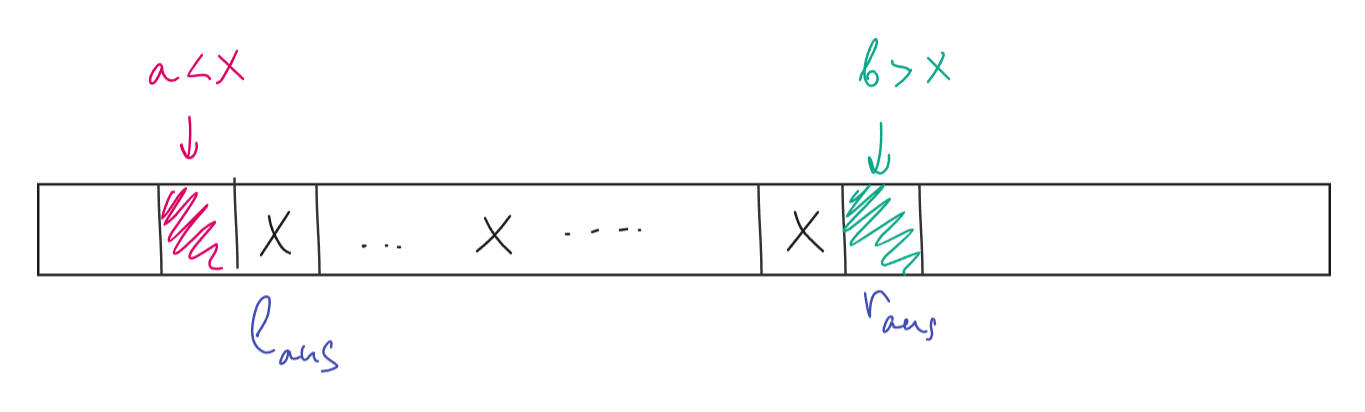
\includegraphics[scale=0.6]{./assets/08-binary-search/1.PNG}
\end{center}


\Subsubsection{STL implementation}

In C++ language we are already provided with the template functions that do the same thing:

\begin{lstlisting}[language=C++]
/* returns iterator (for int* it is a pointer) */
int i = std::lower_bound(a, a + n, x) - a;
int i = std::upper_bound(a, a + n, x) - a;

// For other containers (e.g., std::vector, std::set) that define begin()/end() operations use the following:
std::lower_bound(
    std::begin(container),
    std::end(container),
    element
) //  e.g., for std::vector<T> the return type is std::vector<T>::iterator, i.e. pointer to the element
\end{lstlisting}


\Subsection{Use of a predicate}

We could abstract the implementation even further via searching for a predicate. Predicate is such a function $f: S \to \{0, 1\}$. Then let's consider the predicate $f(i) = if (a_i < x) \ then\ 0\ else\ 1$ - in this case the binary search will find such indicies $l$ and $r$ that satisfy the following:

1. $l + 1 = r$

2. $f(l) = 0$ (i.e. $a_l < x$)

3. $f(r) = 1$ (i.e. $a_r >= x$)

\begin{lstlisting}[language=C++]
int binary_search(int l, int r, int x) {
    while(r - l > 1) {
        int m = (l + r) / 2;
        if (f(m)) r = m; // invariant: f(r) >= x
        else l = m; // invariant f(l) < x
    }
    return r;
}

// If you want to parameterize predicate as well:
// #1: provide a 4th argument as a pointer to a function
// (see: https://www.cprogramming.com/tutorial/function-pointers.html)
int binary_search(int l, int r, int x, bool(*f)(int)) {
    ...
}

// #2: template parameter
template<typename /* or class */ Func>
int binary_search(int l, int r, int x, Func f) {
    ...
}
// possible call:
binary_search(l, r, x, []() { /* predicate impl */ });
\end{lstlisting}

\Subsection{Correctness}

You might already noticed that the functions (arrays are also akin functions, i.e. $a: \{0, 1, .., n-1\}: \mathbb{N} $) over which we apply the binary search algorithm are all monotonic functions, i.e. they comply to $x < y: \ f(x) < f(y)$ (strict monotonically increasing functions; the rest are alike).

\begin{lemma}
    \textit{The binary search algorithm over some range [x, y) is correct iff the considered function $f$ is monotonic over [x, y).}
\end{lemma}



\Subsection{Binary search for functions over $\mathbb{R}$}

It is possible to use the binary search with real numbers as well. Let's consider a problem of \textit{finding square root of} $x$:

\underline{\textbf{Problem statement}}: Given $x \in \mathbb{R}$. Find a value $y \in \mathbb{R}$ so that $y^2 == x$ (for us it is $|y^2 - x| < \varepsilon$):

\begin{lstlisting}[language=C++]
double my_sqrt(double x /* never use 'float' */) {
    double l = 0.0;
    double r = x + 1;

    const dobule EPS = 1e-9; // 10^(-9)

    while(r - l > EPS) {
        double m = (r + l) / 2;
        // Preserve invariant: l^2 <= x, r^2 > x
        if (m*m > x) r = m;
        else l = m;
    }

    return (l + r) / 2;
}
\end{lstlisting}

In the above notice: if $0 < y < 1$ then $y^2 < y$, and if $y \geq 1$ then $y^2 \geq 1$. Thus, for $0 < x < 1$ the corresponding $y$ is greater than $x$, i.e. we select $r = x + 1$.

\begin{example} \textbf{Root of a polynomial} $\mathbf{P(x)}$

    Given a polynomial $P(x)$ of \textbf{an odd degree}, i.e. $\deg{P} = 2k + 1$ with the coerfficient for $x^{2k+1}$ be equal to $1$. There exists a root $x_0 \in \mathbb{R}$, and we need to find it.

    \underline{\textbf{Solution}}:

    We could do that using binary search with any precision $\varepsilon$. First, we need to find points $l$ and $r$, such that: $P(l) < 0$ and $P(r) > 0$ (e.g., $l=-\infty, \ r=+\infty$ - \textbf{MAX\_INT} and \textbf{MIN\_INT} in C++):

    \begin{lstlisting}[language=C++]
    for (l = -1; P(l) >= 0; l *= 2);
    for (r = 1 ; P(r) <= 0; r *= 2);
    \end{lstlisting}

    And finally the root search:

    \begin{lstlisting}[language=C++]
        while (r - l > EPS) {
            double m = (l + r) / 2;
            if (P(m) < 0) l = m; // P(l) < 0
            else r = m; // P(r) >= 0
        }
        return (l + r) / 2;
    \end{lstlisting}

    Actually we need exactly $k := \frac{r-l}{\varepsilon}$ iterations, thus the while-loop could be changed by the for-loop.

\end{example}